\documentclass[a4paper,UTF8]{ctexart}
% \usepackage[utf8]{inputenc}

% Author affiliation
\usepackage{authblk}
% Package for line spacing
\usepackage{setspace}
\renewcommand{\baselinestretch}{2.0} % Double spacing
% Margins
\usepackage[margin=1.25in]{geometry}
% Mathematics
\usepackage{amsmath}
% Tables
\usepackage{tabularx}
\usepackage{booktabs}
% SI units
\usepackage{siunitx}
% Links and referencing within the document
\usepackage[backref]{hyperref}
\hypersetup{hidelinks} 
% Advanced math typesetting
\usepackage{mathtools}
% Graphics
\usepackage{graphicx}
\usepackage{subfig} 
\graphicspath{{./figures}} % Adjust path as needed

\title{这只是一个示例}

\author[1$\dag$]{X}
\author[1$\dag$]{H}
\author[1*]{Q}
\author[1,2]{S}

\affil[1]{R学院,中国}
\affil[2]{A学院,中国}
\affil[*]{通讯作者邮箱}
\affil[$\dag$]{这些作者对本文贡献相同。}

\begin{document}

\maketitle

\begin{abstract}
可重构电池系统由于其灵活且动态可变的拓扑结构,能够适应不同的电池充放电策略,因此为传统电池系统提供了有前途的替代方案。
...
\end{abstract}

\section{方法论}

所提出方法的核心原则是尽可能将RBS中的电池并联,从而最大化输出电流。为了实现这一点,整体过程被分为图 \ref{fig:main} 所示的四个步骤。
...

\begin{figure}[htbp]
    \centering
    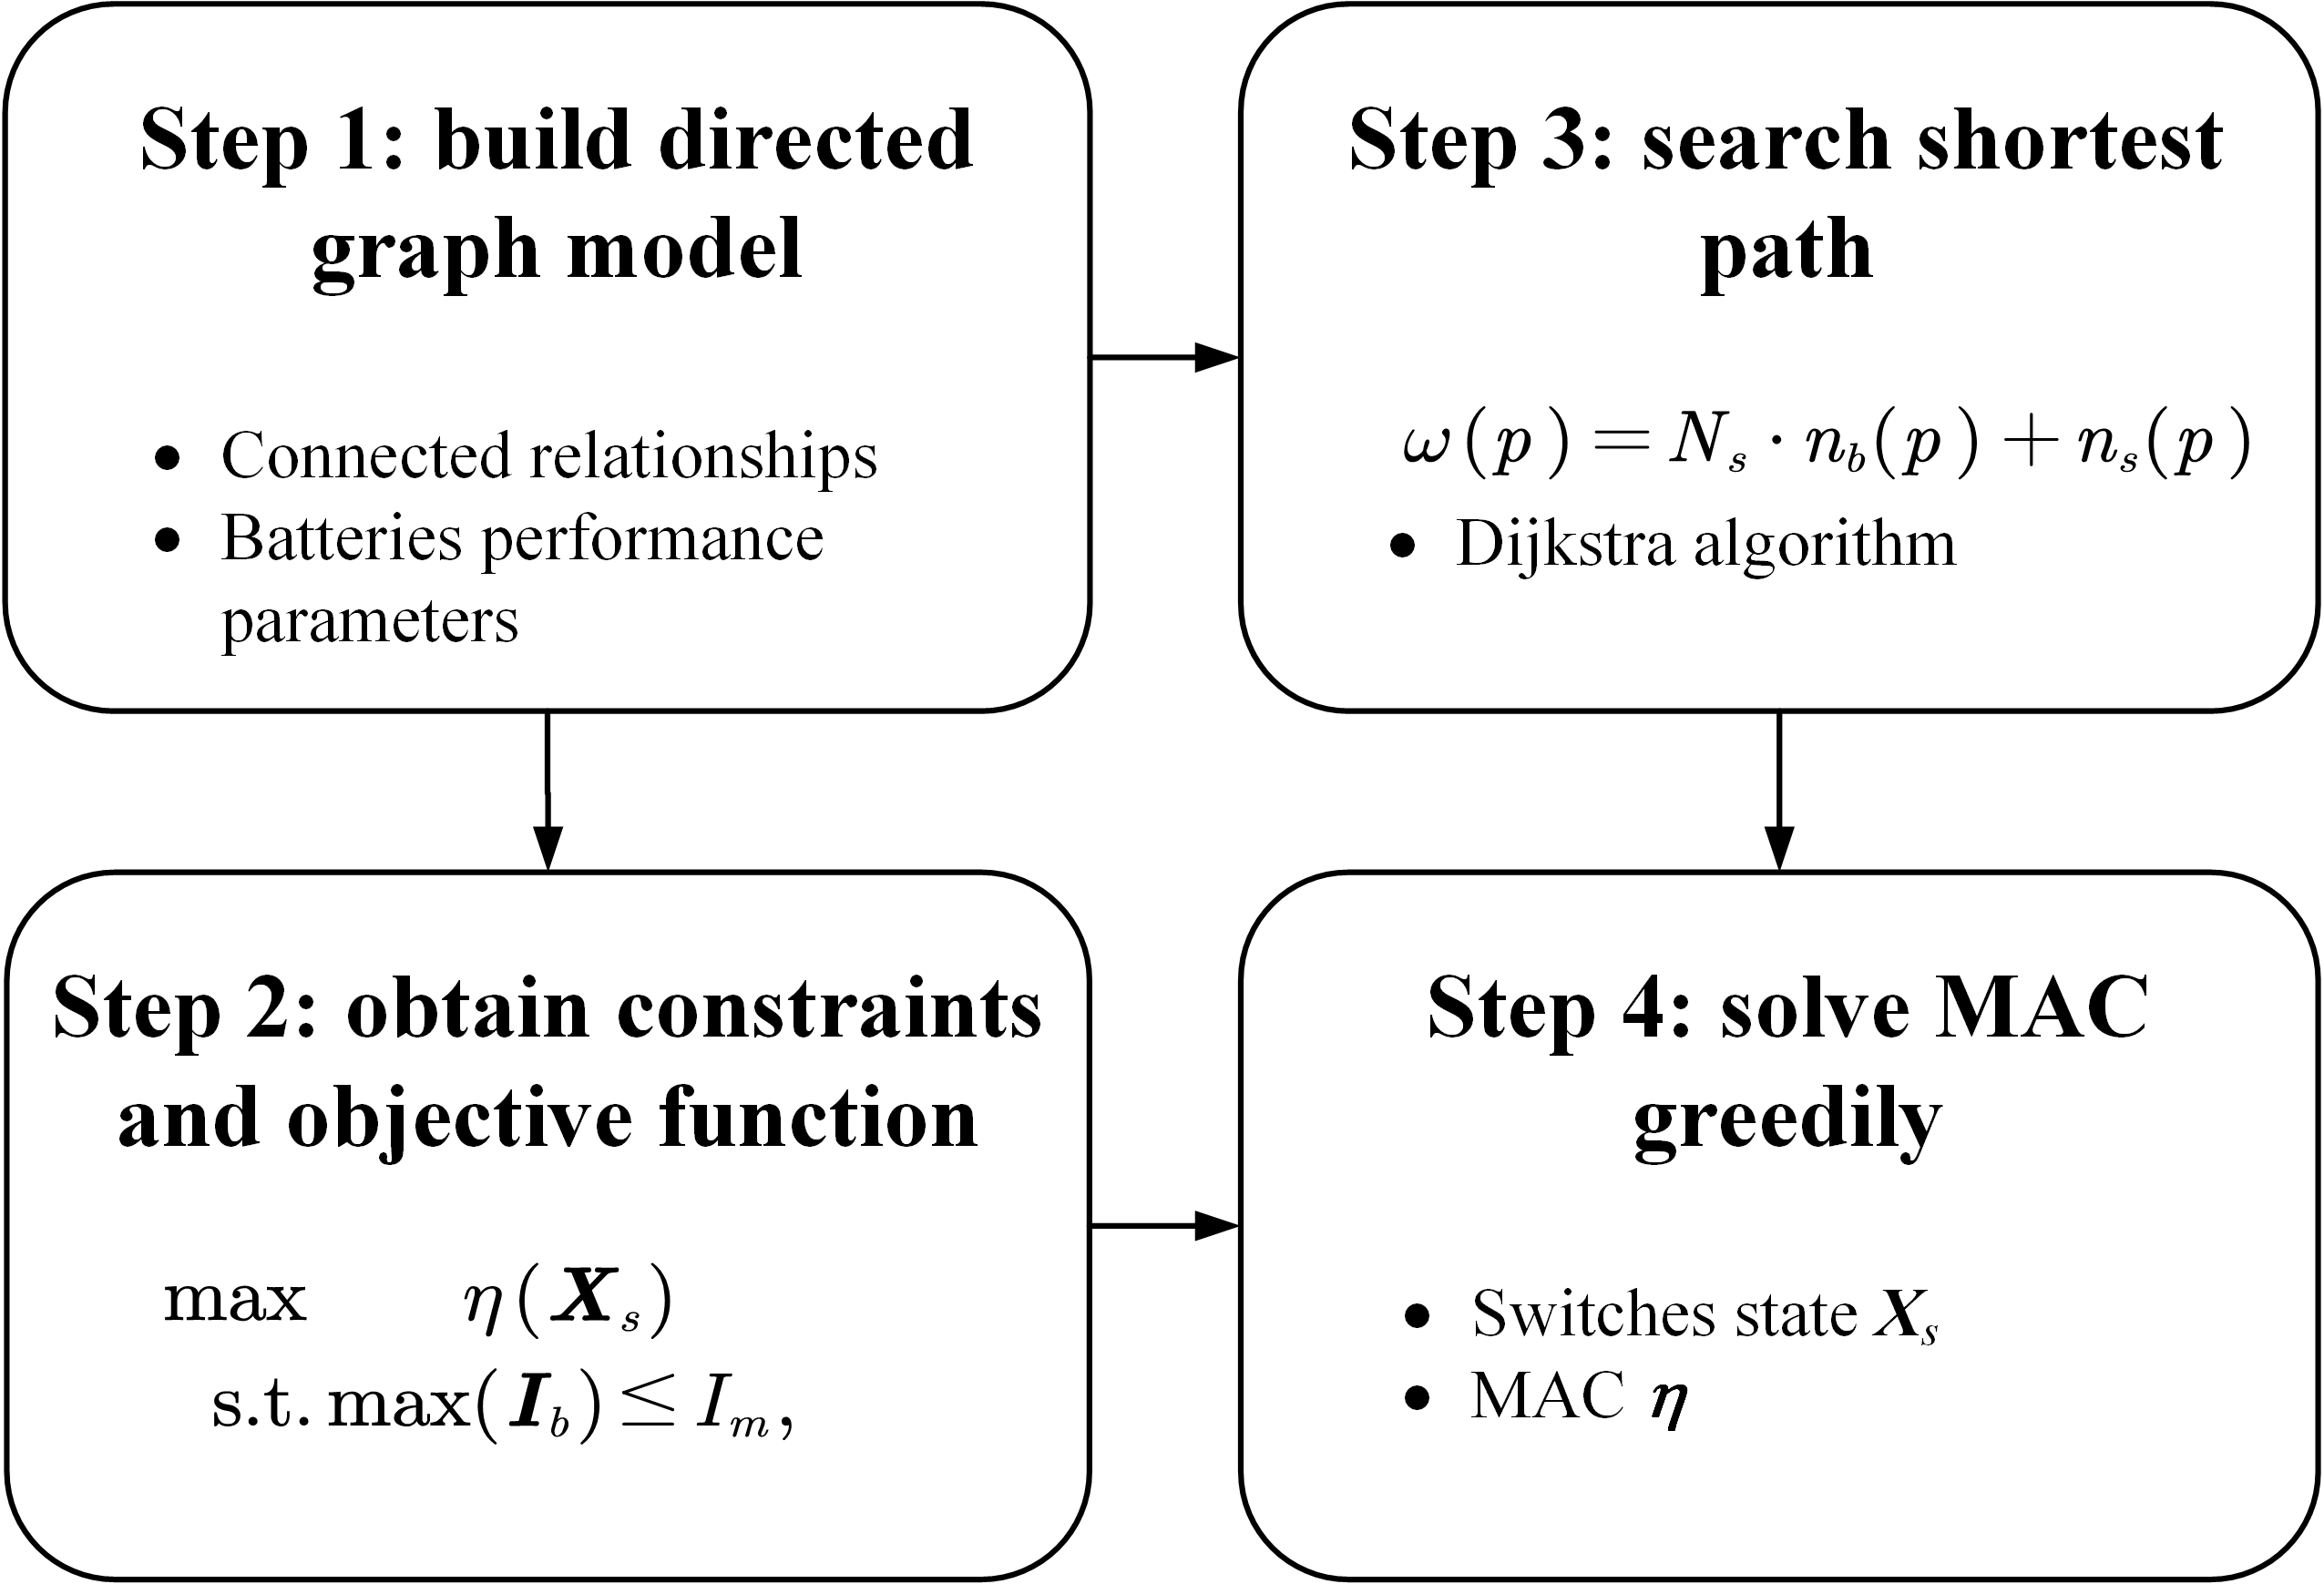
\includegraphics[width=0.8\linewidth]{main.png}
    \caption{
        所提出方法的示意图,包含四个主要步骤。
    }
    \label{fig:main}
\end{figure}

\subsection{有向图模型}

\begin{figure}[htbp]
    \centering
    \subfloat[]{
        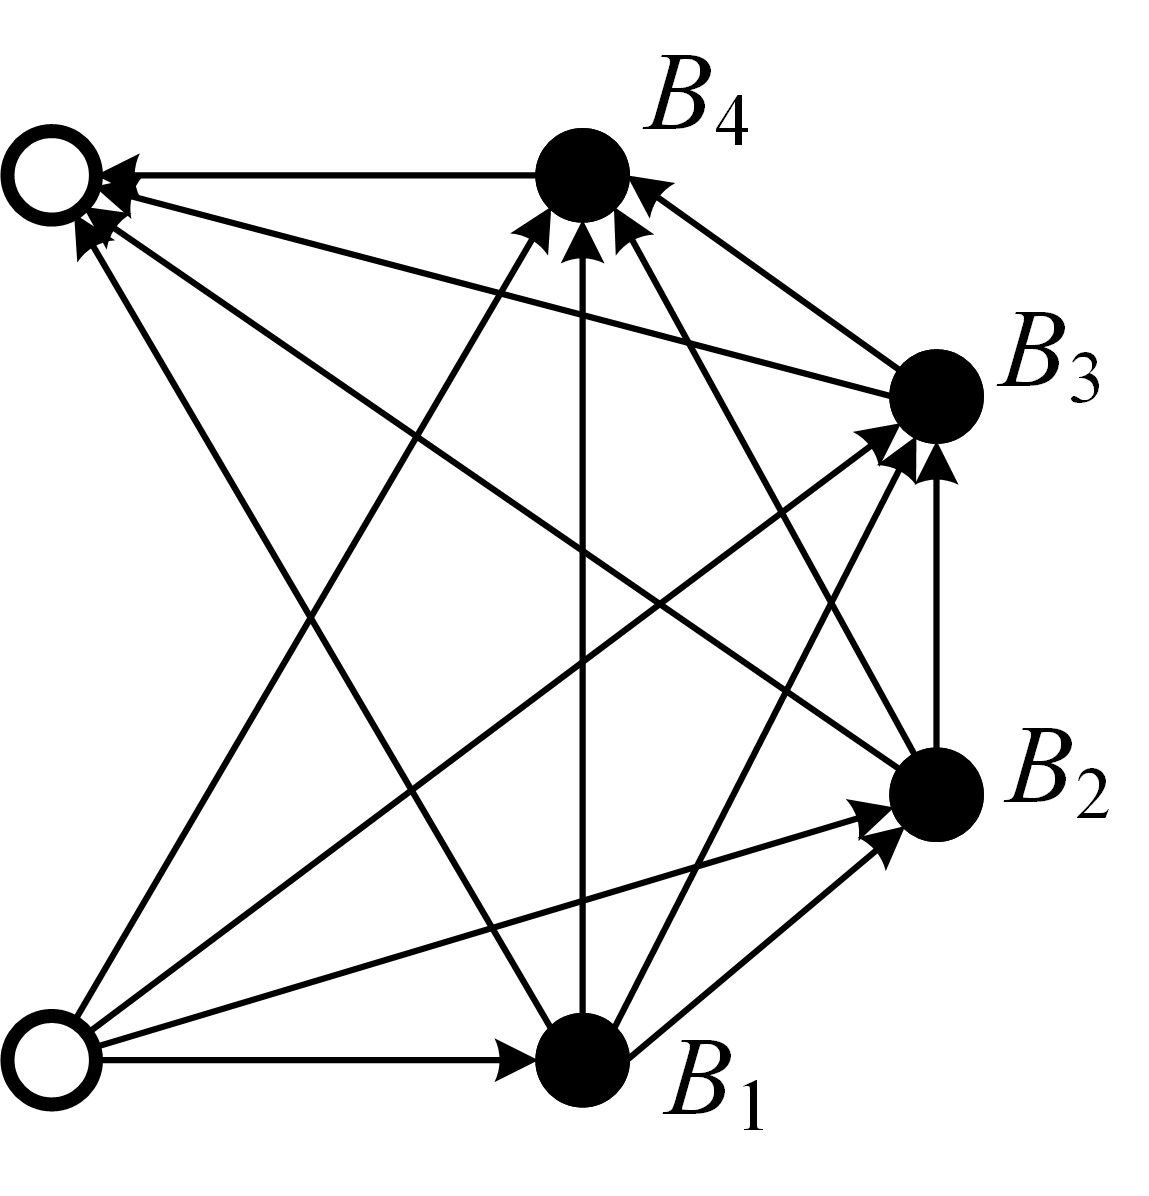
\includegraphics[width=0.31\linewidth]{direct-graph-he.png}
    }
    \subfloat[]{
        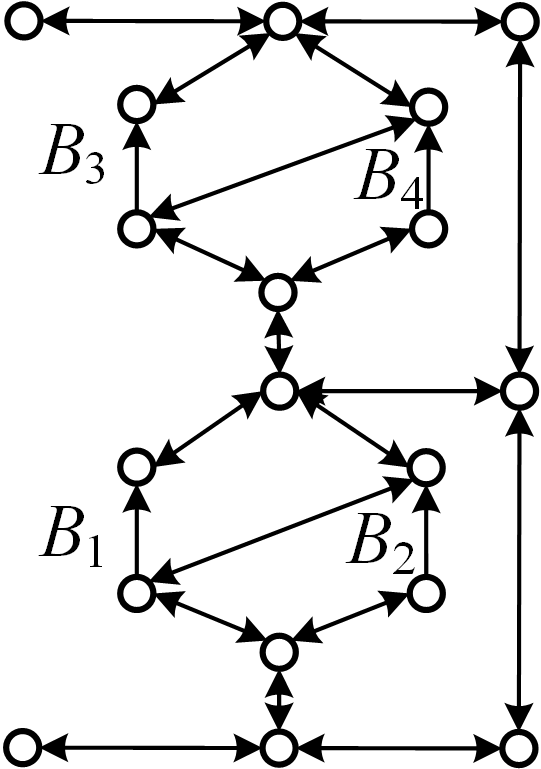
\includegraphics[width=0.23\linewidth]{direct-graph-xu.png}
    }
    \subfloat[]{
        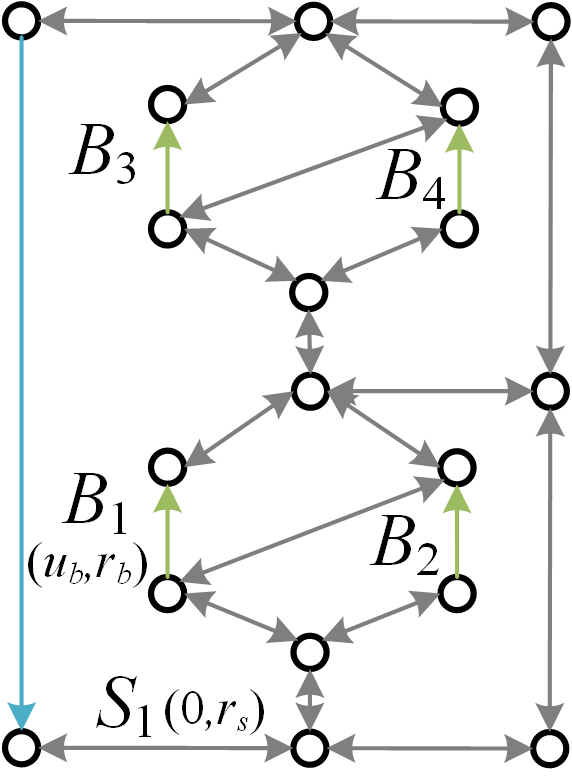
\includegraphics[width=0.24\linewidth]{direct-graph-my.png}
    }
    \\
    \subfloat[]{
        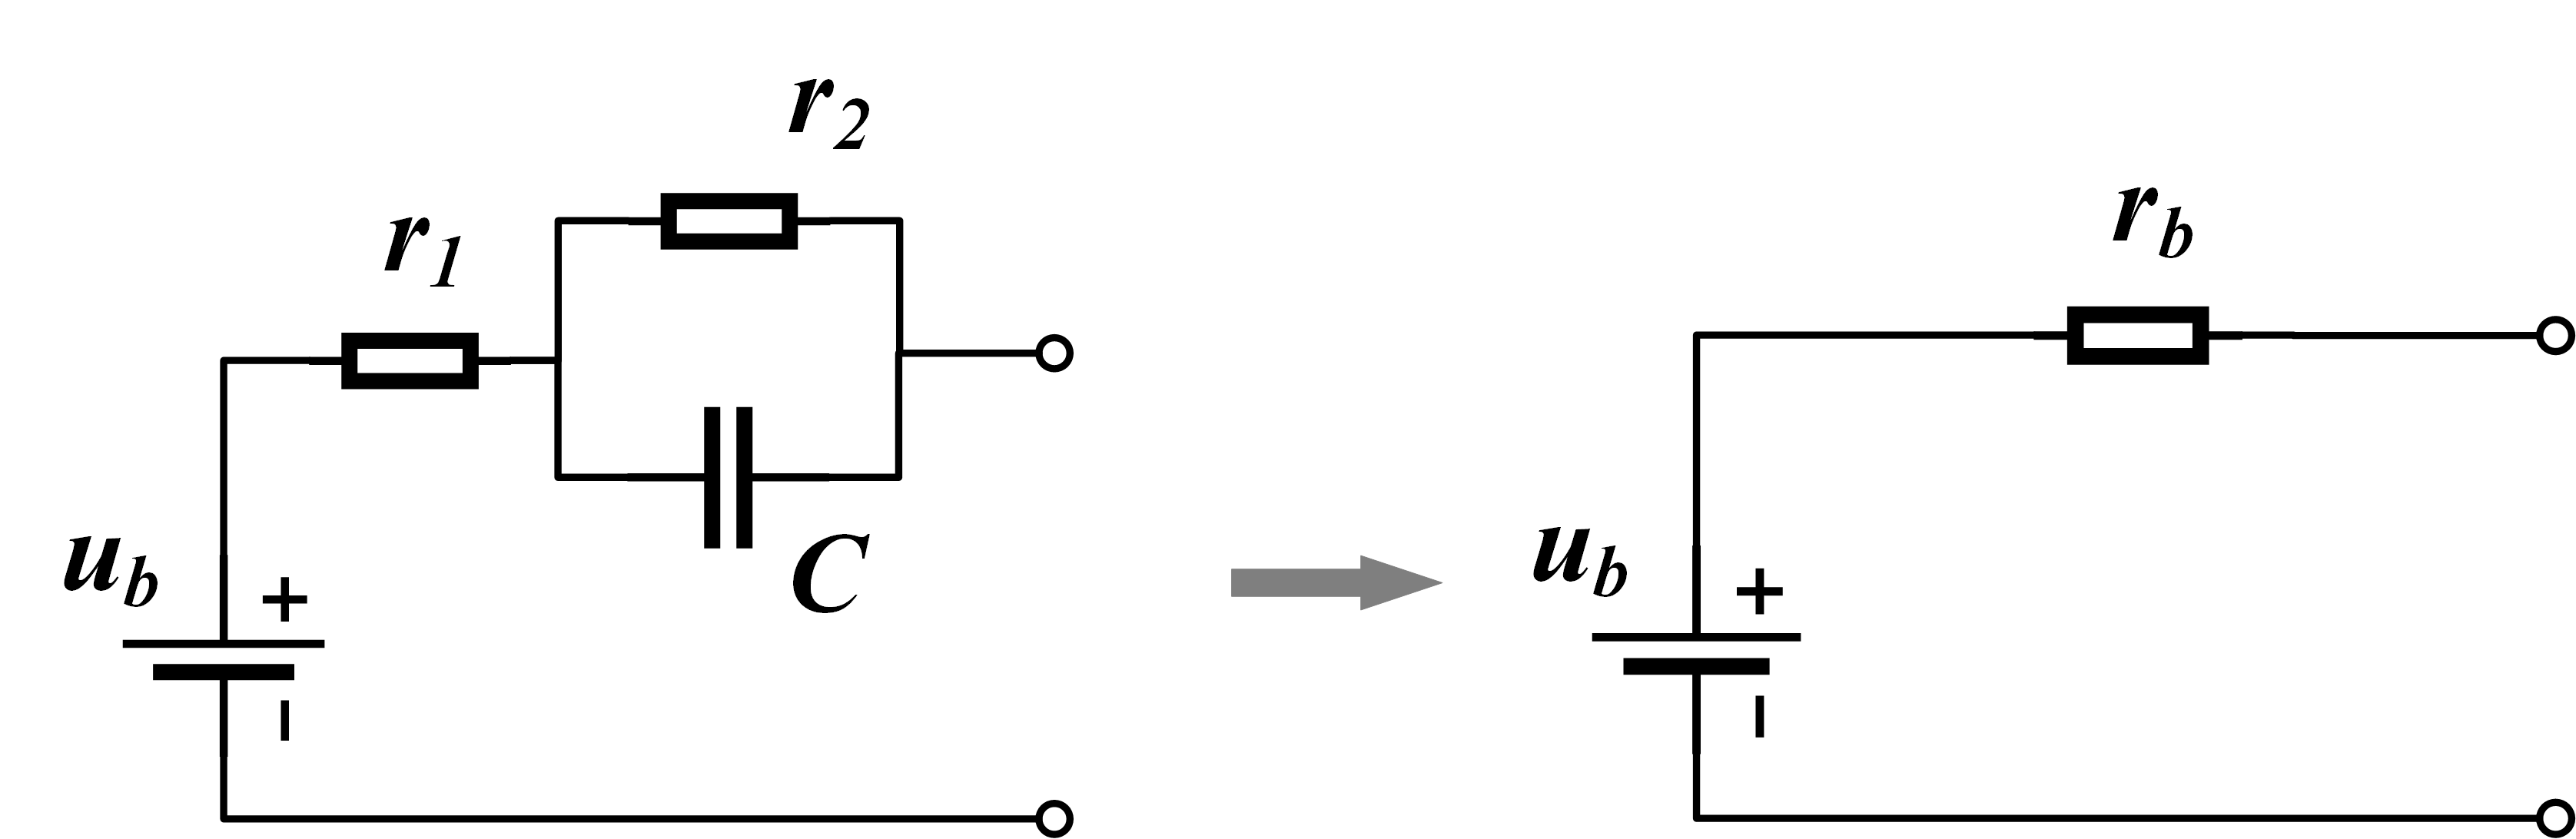
\includegraphics[width=0.8\linewidth]{battery_simple.png}
    }
    \caption{
        所使用的有向图模型:(a) He等人的工作 \cite{heExploringAdaptiveReconfiguration2013},(b) 我们之前的工作,(c) 本文改进的模型。(d) 本方法中电池的等效电路。
    }
    \label{fig:model}
\end{figure}

He等人 \cite{heExploringAdaptiveReconfiguration2013} 提出了RBS的一个抽象有向图模型,其中节点代表电池,边代表配置灵活性,每个顶点的权重对应电池电压 (图 \ref{fig:model}(a))。
...
我们之前提出的有向图模型显著不同于He等人的模型,节点代表电池与开关之间的连接,且有向边代表电池与开关 (图 \ref{fig:model}(b)),从而实现RBS结构与其有向图模型的一一对应。
...
图 \ref{fig:model}(c) 展示了本文使用的改进有向图模型。接下来详细解释了RBS中等效组件的方法及有向图模型的构建。

\subsection{约束条件与目标函数}

首先,有向图模型中的拓扑结构以矩阵 $\boldsymbol{A}$ 的形式表示,该矩阵称为关联矩阵,定义如式 \eqref{eq:A}:
\begin{align}\label{eq:A}
    a_{kl}=
    \begin{cases}
        1,  & \text{边 $l$ 从节点 $k$ 出发},\\
        -1, & \text{边 $l$ 进入节点 $k$},\\
        0,  & \text{其他情况}.
    \end{cases}
\end{align}
对于由 $N$ 个节点和 $N_b+2N_s+1$ 条有向边组成的有向图,关联矩阵 $\boldsymbol{A}$ 是一个 $N\times(N_b+2N_s+1)$ 的矩阵。在该矩阵中,行和列分别表示有向图的节点和边。通过区分RBS中对应每一列的组件,$\boldsymbol{A}$ 可以重写为
\begin{equation}\label{eq:A_bso}
    \boldsymbol{A} =
    \begin{bmatrix}
        \boldsymbol{A}_b & \boldsymbol{A}_s & \boldsymbol{A}_o
    \end{bmatrix},
\end{equation}
其中 $\boldsymbol{A}_b$、$\boldsymbol{A}_s$ 和 $\boldsymbol{A}_o$ 分别是对应电池、开关和外部负载的子矩阵。
...
因此,对于子矩阵 $\boldsymbol{A}_s$,每对代表相同开关的列中仅保留一列。
...
与式 \eqref{eq:A_bso} 类似,$\boldsymbol{\tilde{A}}$ 可以重写为
\begin{equation}\label{eq:A_bso_tilde}
    \boldsymbol{\tilde{A}} =
    \begin{bmatrix}
        \boldsymbol{\tilde{A}}_b & \boldsymbol{\tilde{A}}_s & \boldsymbol{\tilde{A}}_o
    \end{bmatrix}.
\end{equation}


\bibliographystyle{ieeetr}
\bibliography{../ref}

\end{document}
